\chapter{Literature Review}
\label{Chapter2}
\lhead{Chapter 2. \emph{Literature Review}}
\todo{Present a survey of your main approach and an overview of the approaches proposed previously for solving the problem dealt with in this work}

\todo{Identify the practical and research motivation of this work and the literature gaps}

\todo{How convincing is the authors' argument? (Critical response - comparisons with other research, strengths or weaknesses but in relation to your research)}
\section{Optimisation in Air Travel}

In this section, we discuss some common challenges faced by airline companies and demonstrate the importance of optimisation in decision-making for the success and competitiveness of airline companies.

\subsection{Fleet Assignment Problem}


The Fleet Assignment Problem (FAP), as discussed in \cite{airline_fleet_assignement} involves assigning different types of aircraft, to flights based on their capabilities, operational costs, and revenue potential. This decision greatly influences airline revenues and is a vital part of the overall scheduling process. The complexity of FAP is driven by the large number of flights an airline manages daily and its interdependencies with other processes like maintenance and crew scheduling.


\subsection{Crew Scheduling Problem} % (fold)

The Crew Scheduling Problem (CSP), as discussed in \cite{crew_scheduling_problem}, involves assigning crews to a sequence of tasks, each with defined start and end times, with the primary objective of ensuring that all tasks are covered while adhering to regulations on maximum working hours for crew members.

This problem is particularly critical for low-cost airlines, for example in the United Kingdom in 2023, low-cost flights comprise 48\% of the scheduled capacity (total number of seats offered) \cite{lcc_new_norm}, which rely heavily on optimised crew schedules to maintain competitiveness. Efficient crew scheduling is essential not only for low cost carriers and for cost minimisation but also for ensuring operational reliability and flexibility in response to unexpected disruptions.  \cite{ryanair_youtube_report}


\subsection{Disruption Management} % (fold)
\label{sub:disruption management}

Disruptions in airline operations, as noted in \cite{disruption_management}, can occur due to various factors, including crew unavailability, delays from air traffic control, weather conditions, or mechanical failures. Given that flight schedules are typically planned months in advance \cite{flight_scheduling}, effective disruption management is crucial to minimise the impact on passengers and overall airline operations.

The two mains drivers of disruption management are aircraft and crew recovery.
\begin{itemize}
    \item Aircraft recovery: Optimisation tools help manage the complex logistics of matching available aircraft with rescheduled flights, considering factors like airport availability and maintenance requirements.
    \item Crew recovery: Optimisation tools are used to adjust crew schedules, taking into account factors such as legal working hours, crew availability, and the need to cover all flights efficiently. These tools help in developing feasible and compliant crew rosters that adapt to the new flight schedules.
\end{itemize}

These optimisation strategies, supported by advanced software, for instance \cite{inform_software} and \cite{ibs_software}, are crucial for reducing the impact of disruptions and boosting operational resilience in the airline industry.

\subsection{Airline adaptation to new demand} % (fold)
\label{sub:Airline adaptation to new demand}


Airline companies must continuously adapt their schedules to meet evolving market demands, particularly with the growing dominance of leisure travel over business travel, which has introduced new patterns of demand as shown on Figure \ref{fig:European_demand_seasonality} in Europe. This seasonality poses a challenge for airlines as they have to balance high demand during peak seasons with the risk of underutilisation during off-peak times.

\begin{figure}[!ht]
    \centering
    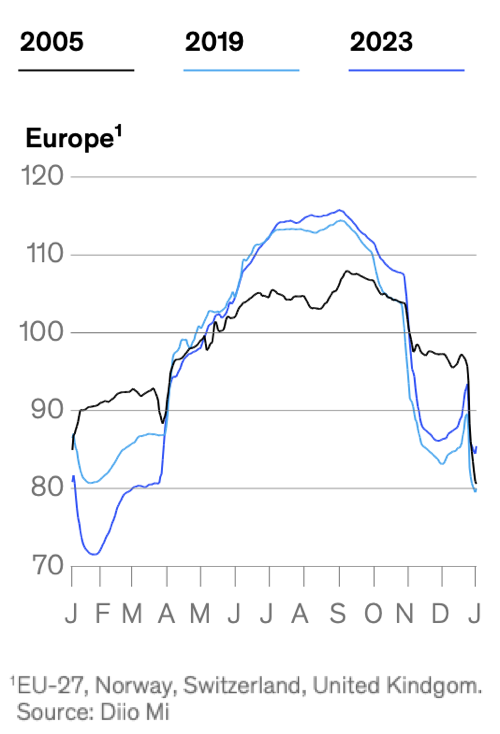
\includegraphics[width=.3\textwidth]{Figures/European Demand.png}
    \caption{European demand seasonality \cite{flight_seasonnality_challenges}}
    \label{fig:European_demand_seasonality}
\end{figure}


Since travel demand varies throughout the year, airlines use a variety of techniques to achieve operational efficiency while maximising revenue \cite{flight_seasonnality_challenges}. For instances, airlines sell nearly 65\% more seats. To ensure their operatios remain efficient during periods of heightened demand, airline companies make the required allowance for additional aircraft and crew by optimisation models that specify priority routes and requirements for additional flights, alongside effective crew rotation management.
\\In contrast, winter months pose a different type of problem where demand drops, which can potentially lead to underutilisation of aircrafts. To manage this, airlines are known to turn to ACMI leasing (agreement between two airlines, where the lessor agrees to provide an aircraft, crew, maintenance and insurance \cite{acmi_def}) during periods of low demand to temporarily reduce fleet size by outsourcing their capacity. Alongside this, they also increase maintenance activities and incentivise crews to take holidays or undergo training to maximise productivity across the operation. Equally, on a year-round basis, airlines apply dynamic pricing algorithms to vary fares in reaction to real-time demand patterns. In high-demand summer months, fares are tactically set so as to maximise revenues from travelers willing to pay more, while in winter, pricing strategies are aimed at stimulating demand with fare reductions to fill seats that otherwise would have gone empty. Such adaptive strategies are critical to the airlines for effectively beating the seasonal ebbs and flows in the travel industry.

%\begin{figure}[!ht]
%    \centering
%    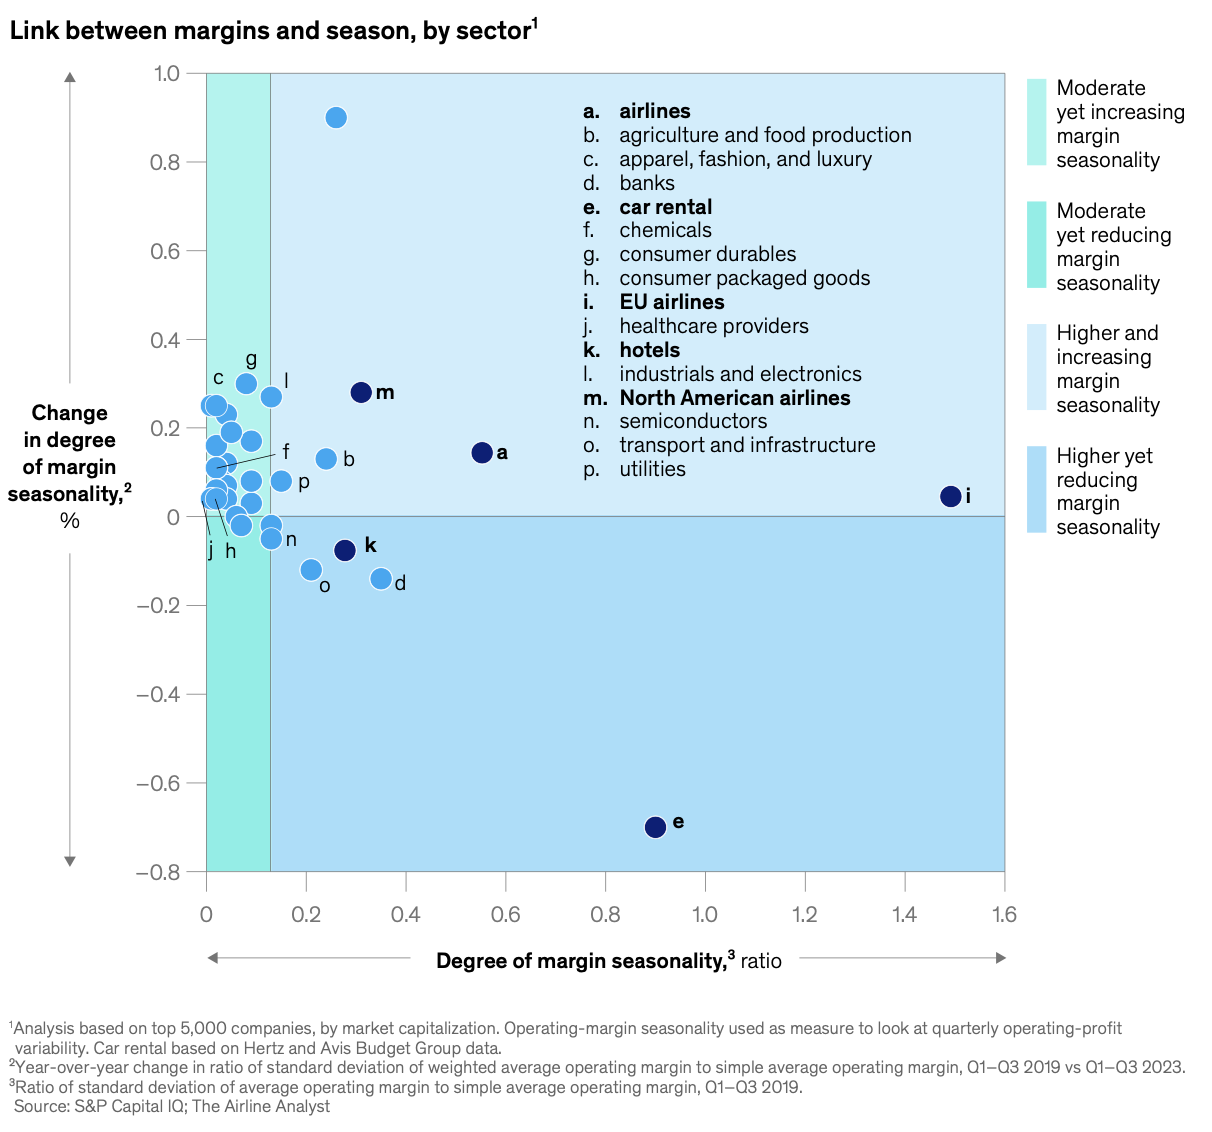
\includegraphics[width=1\textwidth]{Figures/Seasonal margin analysis.png}
%    \caption{Compared with other sectors, airlines exhibit a significant and growing link between margins and seasons.}
%    \label{fig:airline_seasonnality_margin}
%\end{figure}



\newpage
\section{Traveling Salesman problem and its adapation}
\label{sec:TSP}

The Traveling Salesman Problem is a well known problem in the Operational Research and Computer Science fields. A simple description of the TSP is to find the best roundtrip for a saleman that has to travel around a given number of cities while minimising the overall journey's distance.
This problem is characterised as $\mathcal{NP}$-Hard \cite{np_hardness}. This means that there is no known polynomial-time algorithm that can solve all instances of the problem efficiently . Regarding time complexity, if we were to solve it exploring all the possible solutions, the time complexity would have been $\mathcal{O}(\frac{(n-1)!}{2})$ where $n$ represents the number of cities.

\begin{figure}[!ht]
    \centering
    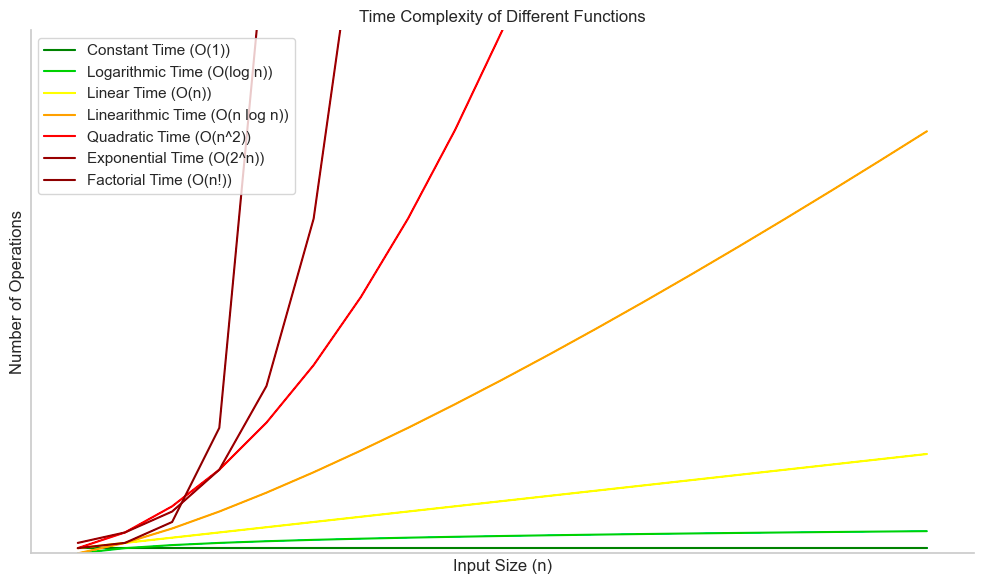
\includegraphics[width=0.8\textwidth]{Figures/NP-hardness - time complexity.png}
    \caption{Time complexity of different functions \cite{time_complexity}}
    \label{fig:time_complexity_comparisons}
\end{figure}

On Figure \ref{fig:time_complexity_comparisons}, different time complexities are compared and demonstrates that the factorial time complexity is the worst. Therefore, these kinds of $\mathcal{NP}$-Hard problem are typically not solved exploiting all the search area but using heuristics algorithms. Heuristics solutions do not guarantee to find the absolute optimal solution but can find near-optimal solutions within more reasonnable timeframes.

The TSP has been studied extensively, and, many variants can be derived from it:

\begin{itemize}
    \item Symmetric TSP (STSP): The distance between cities are symmetric, meaning that the distance to travel from city A to city B is the same as from city B to city A. %\cite{STSP}
    \item Assymetric TSP (ATSP): The distance between cities are assymetric, meaning that the distance to travel from city A to city B is different than the distance to travel from city B to city A.\cite{ASTP}
    \item Multiple TSP (mTSP): Instead of one salesman, multiple salesman are starting from one city, they visit all the cities such that each city is visited exactly once. \cite{mTSP}
    \item Time Window TSP (TWTSP): Each city has to be visited in a defined time slot. \cite{TWTSP}
    \item Price-collection TSP (PCTSP): Not all the cities have to be visited, the goal is to minimise the overall traveler's distance while maximising the price collected earned when visiting a city. \cite{PCTSP}
    \item Stochastic TSP (STSP): The distances between the cities or the cost of travels are stochastic (\i.e random variables) rather than deterministic. \cite{Stochastic_TSP}
    \item Dynamic TSP (DTSP): The problem can change over time, that means that new cities can be added or distances between cities can change while the salesman has already started his journey. \cite{DTSP}
    \item Generalised TSP (GTSP): The cities are grouped into clusters, the goal is to visit exactly one city from each cluster. \cite{GTSP}
    \item Open TSP (OTSP): The traveler does not have to end his journey at the starting city. \cite{OTSP}
\end{itemize}

Multiple algorithms have been developed to address these TSP variants, we can classify them into two categories:

\begin{itemize}
    \item \textbf{Exact Algorithms}: These algorithms aim to find the optimal solution to the TSP by exploring all possible routes or by using mathematical techniques to prune the search space efficiently. Examples include:
          \begin{itemize}
              \item \textbf{Branch and Bound}: This method systematically explores the set of all possible solutions, using bounds to eliminate parts of the search space that cannot contain the optimal solution. It is often used for smaller instances of TSP due to its computational intensity. \cite{branch_and_bound}
              \item \textbf{Cutting Planes}: This technique adds constraints (or cuts) to the TSP formulation iteratively to remove infeasible solutions and converge to the optimal solution. This approach is particularly effective for symmetric TSPs. \cite{cutting_planes}
              \item \textbf{Dynamic Programming}: Introduced by Bellman, this approach breaks down the TSP into subproblems and solves them recursively, which is highly effective for specific TSP variants, though its complexity grows exponentially. \cite{dynamic_programming_tsp}
          \end{itemize}
    \item \textbf{Approximation and Heuristic Algorithms}: These algorithms are designed to find near-optimal solutions within a reasonable time frame, specifically for large-scale problems where exact methods are computationally infeasible. Examples include:
          \begin{itemize}
              \item \textbf{Greedy Algorithms}: These algorithms make a series of locally optimal choices in the hope of finding a global optimum. An example is the Nearest Neighbor algorithm, which selects the nearest unvisited city at each step. \cite{greedy}
              \item \textbf{Genetic Algorithms}: Inspired by the process of natural selection, these algorithms evolve a population of solutions over time, using operations such as mutation and crossover to explore the solution space. \cite{genetic_algorithm}
              \item \textbf{Simulated Annealing}: This probabilistic technique searches for a global optimum by allowing moves to worse solutions based on a temperature parameter that gradually decreases. It is particularly useful for escaping local optima. \cite{simulated_annealing}
              \item \textbf{Ant Colony Optimization}: This metaheuristic is inspired by the foraging behavior of ants and uses a combination of deterministic and probabilistic rules to construct solutions, which qre grqdually refined through updates based on pheromone trails. \cite{ant_colony}
          \end{itemize}
\end{itemize}

Some TSP problems (or its variants) have been solved using other algorithms.

\newpage
\section{The Monte Carlo Tree Search algorithm}

The Monte Carlo Tree Search (MCTS) algorithm can be characterised as less traditionnal than the previously enounced methods in Section \ref{sec:TSP} because MCTS is typically used in games. MCTS' (and its variants)
have been successfully implemented across a range of games, such as Havannah \cite{wiki:board_game},  Amazons \cite{wiki:Game_of_the_Amazons}, Lines of Actions \cite{wiki:Lines_of_Action}, Go, Chess, and Shogi \cite{wiki:Shogi}, establishing it as the state-of-the-art algorithm \cite{havannah}, \cite{amazons}, \cite{lines_of_actions}. It is widely used in board games and is increasingly popular since Google DeepMind developed AlphaGo. AlphaGo is a software that was created to beat the best Go's player in the world.

Go is a board game from China where two players take turns placing black or white stones on a grid. The goal is to capture territory by surrounding empty spaces or the opponent’s stones. Despite its simple rules, Go is a complex game, with countless possible moves and strategies. It is known for its balance between intuition and logic, hence why it has been a significant focus of artificial intelligence research ,\cite{wiki:Go}. In 2016, Lee Sedol \cite{wiki:Lee_Sedol} - the best Go's player in the world was been beaten by AlphaGo 4-1 \cite{alpha_go_documentary}.

MCTS with policy and value networks are at the heart of AlphaGo decision-making process, enabling AlphaGo's to pick the optimal moves in the complex search of Go. \cite{mcts_alpha_go_algorithm}



\subsection{Overview}
The MCTS' process is conceptually straightforward. A tree is built in an incremental and assymatric manner (Figure \ref{fig:Assymetrical_growth_MCTS}).
For every iteration, a selection policy is used to determine which node to select in the tree to perform simulations.
The selection policy, typically balances the exploration  (looking into parts of the tree that have not been visited yet) and the exploitation (looking into parts of the trees that appear to be promising).
Once the node is selected, a simulation - a sequence of available actions, based on a simulation policy, is applied from this node until a terminal condition is reached e.g\ no further actions are possible. \cite{mcts_various_policies}

\begin{figure}[!ht]
    \centering
    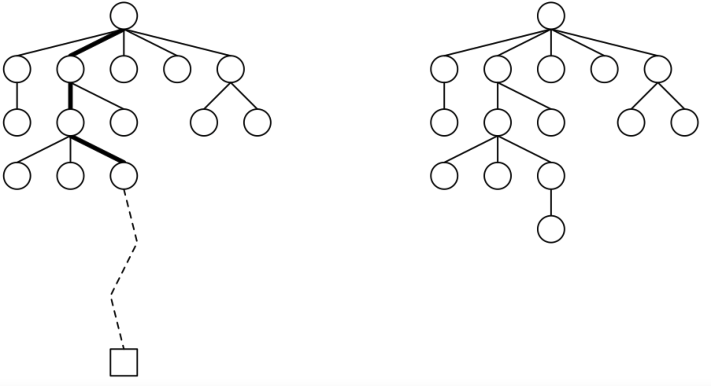
\includegraphics[width=0.5\textwidth]{Figures/assymetric_growth_mcts_tree.png}
    \caption{Assymetrical growth of MCTS - Simulation and Expansion - \cite{mcts_assymetrical_growth}}
    \label{fig:Assymetrical_growth_MCTS}
\end{figure}
\newpage
To ensure a clearer understanding of MCTS algorithm's stages, we will start by exploring a detailed example \cite{example_youtube_mcts}. This example will illustrate each component of the algorithm in action. Furthermore, we will generalise the principles discussed, as the methodology of this paper is built on the application of the MCTS algorithm.


\subsection{Example}
\label{subsub:Example}
Let's say we are given a maximisation problem. When beginning the game, you have two possible actions $a_1$ and $a_2$ from the node $S^{0,0}_0$ in the tree $\mathcal{T}$.
Every node is defined like so: $S^{n_i,t_i}_i$ where $n_i$ represents the number of times node $i$ has been visited, $t_i$ the total score of this node.
Moreover, for every node - we can compute a selection metric, for instance the $UCB1$ value: $UCB1(S^{n_i,t_i}_i)=\bar{V_i} + 2 \sqrt{\frac{\ln N}{n_i}}$ where $\bar{V_i}=\frac{n_i}{t_i}$ represents the average value of the node, $n_i$ the number of times node $i$ has been visited, $N=n_0$ the number of times the root node has been visited (which is also equal to the number of iterations).

Before the first iteration, none node have been visited - $\forall i \in \mathcal{T}, S^{0,0}_{i}$.
\begin{figure}[!ht]
    \centering
    \begin{tikzpicture}[
            root_node/.style={circle, draw=orange!60, fill=orange!5, very thick, minimum size=40},
            visited_node/.style={circle, draw=green!60, fill=green!5, very thick, minimum size=40},
            unvisited_node/.style={circle, draw=gray!60, fill=gray!5, very thick, minimum size=40},
            target_node/.style={circle, draw=green!60, fill=green!5, very thick, minimum size=40},
        ]

        \node[root_node](Root){$S^{0,0}_0$};
        \node[unvisited_node, below left=of Root](S1){$S^{0,0}_1$};
        %\node[target_node, below=of S1, yshift=-1.7cm](Target){};
        \node[unvisited_node, below right=of Root](S2){$S^{0,0}_2$};

        \draw[->] (Root) -- (S1) node[midway, above, xshift=-2mm] {$a_1$};
        \draw[->] (Root) -- (S2) node[midway, above, xshift=2mm] {$a_2$};

        %\draw[->, very thick, decorate, decoration={snake, amplitude=.7mm, segment length=3mm}] (S1) -- (Target);
    \end{tikzpicture}
    \caption{Selection - $I1$}
    \label{fig:Expansion of the tree from the root node}
\end{figure}
At the beginning of $I1$, we have to choose between these two child nodes (or choose between taking $a_1$ or $a_2$). After, we have to calculate the $UCB1$ value for these two nodes and pick the node that maximises the $UCB1$ value (as we are dealing with a maximisation problem).
In Figure \ref{fig:Expansion of the tree from the root node}, neither of these have been visited yet so $USB(S^{0,0}_1)=UCB1(S^{0,0}_2)=\infty$. Hence we decide to choose randomly $S^{0,0}_1$.

$S^{0,0}_1$ is a leaf node that has not been visited - then we can simulate from this node, which means selecting actions from this node based on the simulation policy to a terminal state as shown on Figure \ref{fig:Simulation - $I1$}:

\begin{figure}[!ht]
    \centering
    \begin{tikzpicture}[
            root_node/.style={circle, draw=orange!60, fill=orange!5, very thick, minimum size=40},
            visited_node/.style={circle, draw=green!60, fill=green!5, very thick, minimum size=40},
            unvisited_node/.style={circle, draw=gray!60, fill=gray!5, very thick, minimum size=40},
            target_node/.style={circle, draw=green!60, fill=green!5, very thick, minimum size=40},
        ]

        \node[root_node](Root){$S^{0,0}_0$};
        \node[unvisited_node, below left=of Root](S1){$S^{0,0}_1$};
        \node[target_node, below=of S1, yshift=-1.7cm](Target){20};
        \node[unvisited_node, below right=of Root](S2){$S^{0,0}_2$};

        \draw[->] (Root) -- (S1) node[midway, above, xshift=-2mm] {$a_1$};
        \draw[->] (Root) -- (S2) node[midway, above, xshift=2mm] {$a_2$};

        \draw[->, very thick, decorate, decoration={snake, amplitude=.7mm, segment length=3mm}] (S1) -- (Target);
    \end{tikzpicture}
    \caption{Simulation - $I1$}
    \label{fig:Simulation - $I1$}
\end{figure}

\newpage
The terminal state has a value of 20, we can write that the rollout/simulation from node $S^{0,0}_1$ node is $\mathcal{R}(S^{0,0}_1)=20$ . The final step of $I1$ is backpropagation. Every node that has been visited in the iteration is updated.
Let $\mathcal{N}_{\mathcal{R},j}$ be the indexes of the nodes visited during the $j-th$ iteration of the MCTS:
\begin{itemize}
    \item Before backpropagation:
          \begin{equation}
              \forall i \in \mathcal{N}_{\mathcal{R},j}, S^{n_i,t_i}_{i,old}
          \end{equation}

    \item After backpropagation:
          \begin{equation}
              \forall i \in \mathcal{N}_{\mathcal{R},j}, S^{n_i+1,t_i+\mathcal{R}(S^{n_i,t_i}_{i,old})}_{i,new}
          \end{equation}
\end{itemize}

We can then define a backpropagation function:
\begin{center}
    \centering
    $\begin{array}{ccccc}
            \mathcal{B} & : & \mathcal{N}_{\mathcal{R},j} & \to     & \mathcal{N}_{\mathcal{R},j}                    \\
                        &   & S^{n_i,t_i}_{i}             & \mapsto & S^{n_i+1,t_i+\mathcal{R}(S^{n_i,t_i}_{i})}_{i} \\
        \end{array}$
\end{center}



\newpage
Then, back to the example on Figure \ref{fig:Backpropagation_I1} we update the nodes $\mathcal{B}(S^{0,0}_1)=S^{\mathbf{1},\mathbf{20}}_1$ and $\mathcal{B}(S^{0,0}_0)=S^{\mathbf{1},\mathbf{20}}_0$.
\begin{figure}[!ht]
    \centering
    \begin{tikzpicture}[
            root_node/.style={circle, draw=orange!60, fill=orange!5, very thick, minimum size=40},
            visited_node/.style={circle, draw=green!60, fill=green!5, very thick, minimum size=40},
            unvisited_node/.style={circle, draw=gray!60, fill=gray!5, very thick, minimum size=40},
            target_node/.style={circle, draw=green!60, fill=green!5, very thick, minimum size=40}
        ]

        \node[root_node](Root){$S^{\mathbf{1},\mathbf{20}}_0$};
        \node[unvisited_node, below left=of Root](S1){$S^{\mathbf{1},\mathbf{20}}_1$};
        \node[target_node, below=of S1, yshift=-1.7cm](Target){20};
        \node[unvisited_node, below right=of Root](S2){$S^{0,0}_2$};

        \draw[->] (Root) -- (S1) node[midway, above, xshift=-2mm] {$a_1$};
        \draw[->] (Root) -- (S2) node[midway, above, xshift=2mm] {$a_2$};

        \draw[->, very thick, decorate, decoration={snake, amplitude=.7mm, segment length=3mm}] (Target) -- (S1);
    \end{tikzpicture}
    \caption{Backpropagation - I1}
    \label{fig:Backpropagation_I1}
\end{figure}

The fourth phase of the algorithm has been done for $I1$. Therefore, we can then start the $2^{nd}$ iteration $I2$.
\begin{figure}[!ht]
    \centering
    \begin{tikzpicture}[
            root_node/.style={circle, draw=orange!60, fill=orange!5, very thick, minimum size=40},
            visited_node/.style={circle, draw=green!60, fill=green!5, very thick, minimum size=40},
            unvisited_node/.style={circle, draw=gray!60, fill=gray!5, very thick, minimum size=40},
            target_node/.style={circle, draw=green!60, fill=green!5, very thick, minimum size=40}
        ]

        \node[root_node](Root){$S^{1,20}_0$};
        \node[unvisited_node, below left=of Root](S1){$S^{1,20}_1$};
        %\node[target_node, below=of S1, yshift=-1.7cm](Target){20};
        \node[unvisited_node, below right=of Root](S2){$\mathbf{S^{0,0}_2}$};

        \node[right=2cm of S2, anchor=west] (UCB1) {$UCB(S^{1,20}_1)=20+2 \sqrt{\frac{\ln1}{1}} = 20$};
        \node[below=0.55cm of UCB1, anchor=south] (UCB2) {$UCB(S^{0,0}_2)=\infty$};

        \draw[->] (Root) -- (S1) node[midway, above, xshift=-2mm] {$a_1$};
        \draw[->] (Root) -- (S2) node[midway, above, xshift=2mm] {$a_2$};

        %\draw[->, very thick, decorate, decoration={snake, amplitude=.7mm, segment length=3mm}] (S1) -- (Target);
    \end{tikzpicture}
    \caption{Selection - I2}
    \label{fig:Selection - I2}
\end{figure}
On Figure \ref{fig:Selection - I2}, we can either choose $a_1$ or $a_2$. When a child node has not been visited yet, you pick this node for the Selection or you can compute the $UCB1$ value, it leads to the same conclusion.

\begin{figure}[!ht]
    \centering
    \begin{tikzpicture}[
            root_node/.style={circle, draw=orange!60, fill=orange!5, very thick, minimum size=40},
            visited_node/.style={circle, draw=green!60, fill=green!5, very thick, minimum size=40},
            unvisited_node/.style={circle, draw=gray!60, fill=gray!5, very thick, minimum size=40},
            target_node/.style={circle, draw=green!60, fill=green!5, very thick, minimum size=40},
        ]

        \node[root_node](Root){$S^{\mathbf{2},\mathbf{30}}_0$};
        \node[unvisited_node, below left=of Root](S1){$S^{1,20}_1$};

        \node[unvisited_node, below right=of Root](S2){$S^{\mathbf{1},\mathbf{10}}_2$};
        \node[target_node, below=of S2, yshift=-1.7cm](Target){10};

        \draw[->] (Root) -- (S1) node[midway, above, xshift=-2mm] {$a_1$};
        \draw[->] (Root) -- (S2) node[midway, above, xshift=2mm] {$a_2$};

        \draw[->, very thick, decorate, decoration={snake, amplitude=.7mm, segment length=3mm}] (S2) -- (Target);
    \end{tikzpicture}
    \caption{Simulation and Backpropagation - I2}
    \label{fig:Simulation and Backpropagation - I2}
\end{figure}
\newpage
We can simulate (Figure \ref{fig:Simulation and Backpropagation - I2}) from the chosen node $S^{0,0}_{2}$ and $\mathcal{R}(S^{0,0}_{2})=10$ and backpropagate all the visited nodes: $\mathcal{B}(S^{0,0}_{2})=S^{1,10}_{2}$ and $\mathcal{B}(S^{1,20}_{0})=S^{2,30}_{0}$.
Next, we start the $3^{rd}$ iteration, based on the $UCB1$ score we decide to choose $a_1$.
\begin{figure}[!ht]
    \centering
    \begin{tikzpicture}[
            root_node/.style={circle, draw=orange!60, fill=orange!5, very thick, minimum size=40},
            visited_node/.style={circle, draw=green!60, fill=green!5, very thick, minimum size=40},
            unvisited_node/.style={circle, draw=gray!60, fill=gray!5, very thick, minimum size=40},
            target_node/.style={circle, draw=green!60, fill=green!5, very thick, minimum size=40},
        ]

        \node[root_node](Root){$S^{2,30}_0$};
        \node[unvisited_node, below left=of Root](S1){$S^{1,20}_1$};

        \node[unvisited_node, below right=of Root](S2){$S^{1,10}_2$};
        %\node[target_node, below=of S2, yshift=-1.7cm](Target){10};
        \node[right=5mm of S2, anchor=west, yshift=2mm] (UCB1) {$UCB1(S^{1,20}_1)=\mathbf{21.67}$};
        \node[below=0.55cm of UCB1, anchor=south] (UCB2) {$UCB1(S^{1,10}_2)=11.67$};

        \draw[->] (Root) -- (S1) node[midway, above, xshift=-2mm] {$a_1$};
        \draw[->] (Root) -- (S2) node[midway, above, xshift=2mm] {$a_2$};

        %\draw[->, very thick, decorate, decoration={snake, amplitude=.7mm, segment length=3mm}] (S2) -- (Target);
    \end{tikzpicture}
    \caption{Selection - I3}
    \label{fig:Selection - I3}
\end{figure}


$S^{1,20}_{1}$ is a leaf node and has been visited so we can expand this node.

\begin{figure}[!ht]
    \begin{tikzpicture}[
            root_node/.style={circle, draw=orange!60, fill=orange!5, very thick, minimum size=40},
            visited_node/.style={circle, draw=green!60, fill=green!5, very thick, minimum size=40},
            unvisited_node/.style={circle, draw=gray!60, fill=gray!5, very thick, minimum size=40},
            target_node/.style={circle, draw=green!60, fill=green!5, very thick, minimum size=40},
        ]

        \node[root_node](Root){$S^{3,30}_0$};
        \node[unvisited_node, below left=of Root](S1){$S^{2,20}_1$};
        \node[unvisited_node, below right=of Root](S2){$S^{1,10}_2$};
        \node[unvisited_node, below left=of S1](S3){$S^{1,0}_3$};
        \node[unvisited_node, below right=of S1](S4){$S^{0,0}_4$};

        \node[left=8mm of S1, anchor=east] (UCB1) {$UCB1(S^{2,20}_1)=11.48$};
        \node[below=0.55cm of UCB1, anchor=south] (UCB2) {$UCB1(S^{1,10}_2)=\mathbf{12.10}$};

        %\node[target_node, below=of S3, yshift=-1.7cm](Target){0};

        \draw[->] (Root) -- (S1) node[midway, above, xshift=-2mm] {$a_1$};
        \draw[->] (Root) -- (S2) node[midway, above, xshift=2mm] {$a_2$};
        \draw[->] (S1) -- (S3)   node[midway, above, xshift=-2mm] {$a_3$};
        \draw[->] (S1) -- (S4)   node[midway, above, xshift=2mm] {$a_4$};
        %\draw[->, very thick, decorate, decoration={snake, amplitude=.7mm, segment length=3mm}] (S3) -- (Target);
    \end{tikzpicture}
    \caption{Selection and Expansion - I3}
\end{figure}
\newpage
Based on $UCB1$ score we decide to simulate from $S^{0,0}_3$ on Figure \ref{fig:Simulation and Backpropagation - I3}
\begin{figure}[!ht]
    \centering
    \begin{tikzpicture}[
            root_node/.style={circle, draw=orange!60, fill=orange!5, very thick, minimum size=40},
            visited_node/.style={circle, draw=green!60, fill=green!5, very thick, minimum size=40},
            unvisited_node/.style={circle, draw=gray!60, fill=gray!5, very thick, minimum size=40},
            target_node/.style={circle, draw=green!60, fill=green!5, very thick, minimum size=40},
        ]

        \node[root_node](Root){$S^{\mathbf{3},30}_0$};
        \node[unvisited_node, below left=of Root](S1){$S^{\mathbf{2},20}_1$};
        \node[unvisited_node, below right=of Root](S2){$S^{\mathbf{2},10}_2$};
        \node[unvisited_node, below left=of S1](S3){$S^{\mathbf{1},0}_3$};
        \node[unvisited_node, below right=of S1](S4){$S^{0,0}_4$};

        \node[target_node, below=of S3, yshift=-1.7cm](Target){0};

        \draw[->] (Root) -- (S1) node[midway, above, xshift=-2mm] {$a_1$};
        \draw[->] (Root) -- (S2) node[midway, above, xshift=2mm] {$a_2$};
        \draw[->] (S1) -- (S3)   node[midway, above, xshift=-2mm] {$a_3$};
        \draw[->] (S1) -- (S4)   node[midway, above, xshift=2mm] {$a_4$};
        \draw[->, very thick, decorate, decoration={snake, amplitude=.7mm, segment length=3mm}] (Target) -- (S3);
    \end{tikzpicture}
    \caption{Simulation and Backpropagation - I3}
    \label{fig:Simulation and Backpropagation - I3}
\end{figure}
\newpage
This is the fourth iteration $I4$ represented on Figure \ref{fig:Selection - Simulation - Backpropagation - I4}:
\begin{figure}[!ht]
    \centering
    \begin{tikzpicture}[
            root_node/.style={circle, draw=orange!60, fill=orange!5, very thick, minimum size=40},
            visited_node/.style={circle, draw=green!60, fill=green!5, very thick, minimum size=40},
            unvisited_node/.style={circle, draw=gray!60, fill=gray!5, very thick, minimum size=40},
            target_node/.style={circle, draw=green!60, fill=green!5, very thick, minimum size=40},
        ]

        \node[root_node](Root){$S^{\mathbf{4,44}}_0$};
        \node[unvisited_node, below left=of Root](S1){$S^{2,20}_1$};
        \node[unvisited_node, below right=of Root](S2){$S^{\mathbf{2},\mathbf{24}}_2$};
        \node[unvisited_node, below left=of S1](S3){$S^{1,0}_3$};
        \node[unvisited_node, below=of S1](S4){$S^{0,0}_4$};
        \node[unvisited_node, below left=of S2](S5){$S^{\mathbf{1},\mathbf{14}}_5$};
        \node[unvisited_node, below right=of S2](S6){$S^{0,0}_6$};


        \node[target_node, below=of S5, yshift=-1.7cm](Target){14};

        \draw[->] (Root) -- (S1) node[midway, above, xshift=-2mm] {$a_1$};
        \draw[->] (Root) -- (S2) node[midway, above, xshift=2mm] {$a_2$};
        \draw[->] (S1) -- (S3)   node[midway, above, xshift=-2mm] {$a_3$};
        \draw[->] (S1) -- (S4)   node[midway, above, xshift=3mm] {$a_4$};
        \draw[->] (S2) -- (S5) node[midway, above, xshift=-2mm] {$a_5$};
        \draw[->] (S2) -- (S6) node[midway, above, xshift=2mm] {$a_6$};

        \draw[->, very thick, decorate, decoration={snake, amplitude=.7mm, segment length=3mm}] (S5) -- (Target);
    \end{tikzpicture}
    \caption{Selection - Simulation - Backpropagation - I4}
    \label{fig:Selection - Simulation - Backpropagation - I4}
\end{figure}

The MCTS algorithm can either be stopped because you are running out of time or because you have no more available actions. For instance, if we were to stop at this stage of the algorithm, the best action to undertake is $a_2$ because it has the higher average value: $\bar{V_1}=\frac{20}{2} \le \bar{V_2}=\frac{24}{2}$.

\subsection{The different parameters in the MCTS}


\subsection{Selection policy}
\cite{different_selection_policies}
\begin{itemize}
    \item \textbf{Upper Confidence Bound (UCB):}
          \begin{itemize}
              \item \textit{Description}: UCB is a popular selection policy in MCTS that balances exploration and exploitation using a mathematical formulation that considers both the average reward of a node and the uncertainty of that reward.
              \item \textit{Trade-offs}:
                    \begin{itemize}
                        \item \textbf{Exploration vs. Exploitation}: UCB adjusts the balance between exploring less-visited nodes and exploiting nodes with high rewards.
                        \item \textbf{Parameter Sensitivity}: The performance of UCB depends on the constant \(C_p\) in its formula, which controls the level of exploration.
                        \item \textbf{Children's Count}: UCB can lead to varying numbers of children being explored, depending on the setting of \(C_p\).
                    \end{itemize}
          \end{itemize}

    \item \textbf{UCB1-Tuned:}
          \begin{itemize}
              \item \textit{Description}: A variation of UCB that dynamically adjusts the exploration term based on the variance of rewards, making it more adaptive to different scenarios.
              \item \textit{Trade-offs}:
                    \begin{itemize}
                        \item \textbf{Adaptivity}: UCB1-Tuned can adapt to the variance in the rewards, potentially leading to better performance in complex environments.
                        \item \textbf{Computational Cost}: The added complexity in adjusting the exploration term may lead to higher computational costs.
                        \item \textbf{Children's Count}: This policy may result in fewer nodes being selected for expansion when the variance is low, focusing more on exploitation.
                    \end{itemize}
          \end{itemize}

    \item \textbf{Single-Player (SP-MCTS):}
          \begin{itemize}
              \item \textit{Description}: A variant of MCTS specifically designed for single-player scenarios, incorporating a third term in the UCB formula to account for the uncertainty in node values.
              \item \textit{Trade-offs}:
                    \begin{itemize}
                        \item \textbf{Exploration of Uncertainty}: SP-MCTS inflates the uncertainty term for less-visited nodes, which can lead to more thorough exploration in single-player settings.
                        \item \textbf{Focus on Strong Lines}: This policy tends to favor strong lines of play, potentially neglecting less promising but necessary exploratory paths.
                        \item \textbf{Children's Count}: Tends to explore a wider range of children nodes, balancing between known strong strategies and potential new solutions.
                    \end{itemize}
          \end{itemize}

    \item \textbf{Bayesian UCT:}
          \begin{itemize}
              \item \textit{Description}: Bayesian UCT integrates Bayesian statistics into the selection policy, allowing for a probabilistic approach to balancing exploration and exploitation.
              \item \textit{Trade-offs}:
                    \begin{itemize}
                        \item \textbf{Probabilistic Exploration}: Bayesian UCT provides a more nuanced exploration strategy by considering prior knowledge and updating beliefs as more information is gathered.
                        \item \textbf{Complexity}: The Bayesian approach can be computationally expensive, especially in large search spaces.
                        \item \textbf{Children's Count}: The number of children explored under Bayesian UCT can be influenced by the prior distributions used, potentially leading to more focused exploration in areas of high uncertainty.
                    \end{itemize}
          \end{itemize}
\end{itemize}

\section{Selection Policies}
\label{sub:selection_policies_litterature}
\subsection{Single-Player MCTS (SP-MCTS)}
Single-Player MCTS (SP-MCTS) is an adaptation of the Monte Carlo Tree Search (MCTS) algorithm specifically designed for single-player games. SP-MCTS modifies the standard Upper Confidence Bounds (UCB) formula by adding a third term to account for the possible deviation of a node's value, adjusting the standard deviation for infrequently visited nodes to better estimate rewards.

The modified UCB formula used in SP-MCTS is:
\begin{equation}
    rD \frac{\sigma^2}{n_i} + n_i,
\end{equation}
where \( \sigma^2 \) is the variance of the node's simulation results, \( n_i \) is the number of visits to the node, and \( D \) is a constant that inflates the standard deviation for less frequently visited nodes.

Key enhancements in SP-MCTS include:
\begin{itemize}
    \item \textbf{Heuristic-Guided Default Policy}: A heuristic is used to guide simulations, improving the efficiency of the search process.
    \item \textbf{Meta-Search}: To avoid getting stuck in local maxima, SP-MCTS periodically restarts with different random seeds and stores the best solution across runs.
    \item \textbf{Maximization Tracking}: By tracking maximum simulation results, SP-MCTS ensures that strong lines of play are not overshadowed by weaker ones.
\end{itemize}

\subsection{UCB1-Tuned}
UCB1-Tuned is an enhancement of the standard UCB1 algorithm, designed to fine-tune the balance between exploration and exploitation in MCTS. This approach adjusts the exploration term based on sample variance, providing a more accurate trade-off in dynamic environments.

The UCB1-Tuned formula is:
\begin{equation}
    \sqrt{\frac{\ln n}{n_j}} \cdot \min\left(1, V_j(n_j)\right),
\end{equation}
where:
\begin{equation}
    V_j(n_j) = \frac{1}{2} \sum_{s=1}^{n_j} \left(X_{j,s}^2 - X_j\right) + \frac{\sqrt{2 \ln t}}{s},
\end{equation}
and \( n_j \) is the number of times the machine \( j \) has been played, \( X_{j,s} \) is the reward for each play, and \( t \) is the total number of plays.

Notable applications of UCB1-Tuned include:
\begin{itemize}
    \item \textbf{Improved Exploration-Exploitation Trade-off}: UCB1-Tuned replaces the upper confidence bound term with one that accounts for variance, leading to better decision-making.
    \item \textbf{Domain Applications}: The UCB1-Tuned approach has been successfully applied in games like Go and real-time environments, showing superior performance compared to the standard UCB1.
\end{itemize}

\subsection{Upper Confidence Bounds for Trees (UCT)}
UCT is the foundational algorithm for MCTS, combining Monte Carlo simulations with the UCB1 algorithm for selecting actions during the search process. UCT ensures a balance between exploring new actions and exploiting known good ones.

The UCB1 formula used in UCT is:
\begin{equation}
    X_j + C_p \sqrt{\frac{\ln N}{n_j}},
\end{equation}
where \( X_j \) is the average reward from action \( j \), \( C_p \) is the exploration constant, \( N \) is the total number of simulations, and \( n_j \) is the number of times action \( j \) has been tried.

Core components of UCT:
\begin{itemize}
    \item \textbf{Exploration-Exploitation Balance}: UCT employs the UCB1 formula to manage the trade-off between exploration and exploitation during tree growth.
    \item \textbf{Tree Growth Mechanism}: UCT builds a search tree dynamically, where nodes are expanded based on the outcomes of simulations, continuously refining the action-value estimates.
\end{itemize}

\subsection{Bayesian UCT}
Bayesian UCT introduces Bayesian methods into the UCT framework to improve the estimation of node values and their uncertainties, especially in scenarios with limited simulation trials.

The Bayesian tree policy can be represented as:
\begin{equation}
    B_i = \mu_i + \frac{\sqrt{2 \ln N}}{n_i},
\end{equation}
where \( \mu_i \) is the mean of an extremum (minimax) distribution \( P_i \), and \( n_i \) is the number of visits to the node \( i \).

An alternative Bayesian UCT formula is:
\begin{equation}
    B_i = \mu_i + \sigma_i \cdot \sqrt{\frac{2 \ln N}{n_i}},
\end{equation}
where \( \sigma_i \) is the square root of the variance of \( P_i \).

Key strategies in Bayesian UCT:
\begin{itemize}
    \item \textbf{Bayesian Tree Policies}: Two tree policies are proposed—one that maximizes mean rewards and another that maximizes mean plus variance, with the latter often showing superior performance.
    \item \textbf{Improved Convergence}: Bayesian UCT demonstrates better convergence properties compared to standard UCT, particularly when accurate prior information is available.
\end{itemize}

\subsubsection{Different nodes}